\documentclass[11pt, a4paper]{article}

\usepackage[utf8]{inputenc}
\usepackage[T1]{fontenc}
\usepackage[a4paper, margin=2.5cm]{geometry}
\usepackage{enumitem}
\setlist[itemize]{label=-}
\usepackage{hyperref}
\usepackage{graphicx}
\usepackage{array}
\usepackage{booktabs}
\usepackage{float}
\usepackage{tikz}
\usetikzlibrary{positioning, fit, arrows.meta, calc}
\usepackage{pgfgantt}

% Nomes em português (sem depender do babel)
\renewcommand{\figurename}{Figura}
\renewcommand{\tablename}{Tabela}
\renewcommand{\refname}{Referências}
\renewcommand{\abstractname}{Resumo}

\title{\textbf{Implementação de Mecanismos de QoS usando VNFs: Proposta de Projeto}}
\author{
  \textbf{GRUPO 6} \\[0.4cm]
  Ivo Costa Sousa -- \texttt{pg63976} \\[0.15cm]
  João Afonso Almeida Sousa -- \texttt{pg62405} \\[0.15cm]
  João Carlos Teixeira Neiva -- \texttt{pg63978} \\[0.15cm]
}
\date{Novembro de 2026}

\begin{document}

\maketitle

\begin{abstract}
\textit{Esta proposta, no âmbito do Trabalho Prático 3 da Unidade Curricular de Qualidade de Serviço na Internet, descreve um sistema de QoS baseado em Funções de Rede Virtualizadas (VNFs): uma cadeia de três VNFs no caminho de dados (controlo de acesso, classificação e controlo de tráfego) e uma VNF de monitorização, emuladas em Containernet sobre uma topologia semelhante à de um ISP. Apresentam-se a topologia, a política DiffServ, as ferramentas, os cenários de teste e o planeamento.}
\end{abstract}

\section{Objetivos}
O projeto cobre os cinco aspetos de QoS do enunciado (classificação, controlo de acesso, policiamento, agendamento e monitorização), cada um implementado como VNF num contentor Docker. Com a ligação de acesso de 10~Mbit/s congestionada, a cadeia deve garantir:
\begin{itemize}
    \item \textbf{VoIP:} atraso num sentido inferior a 150~ms (ITU-T G.114~\cite{g114}), \textit{jitter} inferior a 30~ms e perdas inferiores a 1\%.
    \item \textbf{Vídeo:} débito de pelo menos 4~Mbit/s com perdas inferiores a 1\%.
    \item \textbf{Best effort:} utilização da capacidade restante sem esgotar as outras classes.
    \item \textbf{Tráfego não autorizado:} 100\% descartado na primeira VNF da cadeia.
\end{itemize}
Cada meta é medida com as VNFs em modo de simples encaminhamento (sem QoS) e com a cadeia ativa, de forma a quantificar o ganho e o custo de cada função.

\section{Topologia}
A topologia imita um ISP: a LAN de clientes chega à LAN de servidores através da cadeia de VNFs, de uma ligação de acesso de 10~Mbit/s e de dois \textit{routers} de borda (Figura~\ref{fig:topologia}). Todos os nós são contentores Docker criados pelo \textit{script} \texttt{topologia.py}, que também configura endereços, rotas e as características das ligações (\texttt{tbf} no acesso e \texttt{netem} no núcleo). O plano de endereçamento completo consta do \texttt{README} do repositório.

\begin{figure}[htbp]
\centering
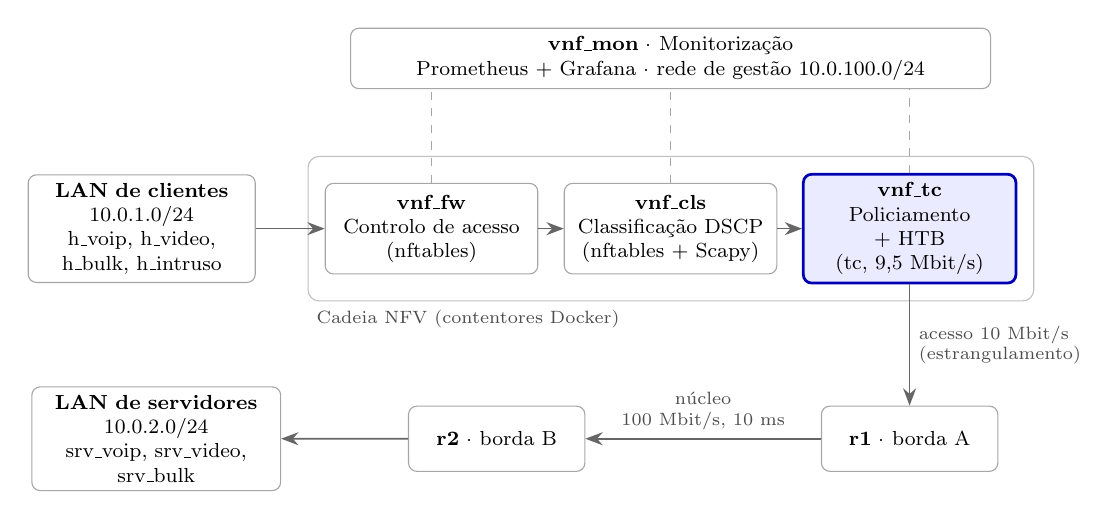
\begin{tikzpicture}[scale=0.92, transform shape,
    font=\footnotesize,
    box/.style={draw=gray!70, rounded corners=3pt, align=center, text width=2.9cm, minimum height=1.25cm, fill=white},
    vnf/.style={box, text width=2.7cm},
    hot/.style={vnf, draw=blue!70!black, line width=1pt, fill=blue!8},
    data/.style={-{Stealth[length=2.2mm]}, gray!80!black, line width=0.6pt},
    mgmt/.style={dashed, gray!70, line width=0.5pt},
    lbl/.style={font=\scriptsize, text=gray!60!black}
]
    % Linha 1: clientes e cadeia NFV
    \node[box] (lanc) at (0,0) {\textbf{LAN de clientes}\\10.0.1.0/24\\h\_voip, h\_video,\\h\_bulk, h\_intruso};
    \node[vnf] (fw)  at (4.0,0) {\textbf{vnf\_fw}\\Controlo de acesso\\(nftables)};
    \node[vnf] (cls) at (7.3,0) {\textbf{vnf\_cls}\\Classificação DSCP\\(nftables + Scapy)};
    \node[hot] (tc)  at (10.6,0) {\textbf{vnf\_tc}\\Policiamento + HTB\\(tc, 9,5~Mbit/s)};
    \node[draw=gray!50, rounded corners=4pt, inner sep=6pt, fit=(fw)(cls)(tc), label={[lbl, anchor=north west]south west:Cadeia NFV (contentores Docker)}] (nfv) {};

    % Monitorização por cima
    \node[box, text width=8.6cm, minimum height=0.8cm] (mon) at (7.3,2.35) {\textbf{vnf\_mon} · Monitorização\\Prometheus + Grafana · rede de gestão 10.0.100.0/24};

    % Linha 2: núcleo e servidores (fluxo da direita para a esquerda)
    \node[box, text width=2.2cm, minimum height=0.9cm] (r1) at (10.6,-2.9) {\textbf{r1} · borda A};
    \node[box, text width=2.2cm, minimum height=0.9cm] (r2) at (4.9,-2.9) {\textbf{r2} · borda B};
    \node[box, text width=3.2cm] (lans) at (0.2,-2.9) {\textbf{LAN de servidores}\\10.0.2.0/24\\srv\_voip, srv\_video,\\srv\_bulk};

    % Caminho de dados
    \draw[data] (lanc) -- (fw);
    \draw[data] (fw) -- (cls);
    \draw[data] (cls) -- (tc);
    \draw[data] (tc.south) -- node[lbl, right, align=left] {acesso 10~Mbit/s\\(estrangulamento)} (r1.north);
    \draw[data] (r1) -- node[lbl, above, align=center] {núcleo\\100~Mbit/s, 10~ms} (r2);
    \draw[data] (r2) -- (lans);

    % Gestão
    \draw[mgmt] (fw.north) -- (fw.north |- mon.south);
    \draw[mgmt] (cls.north) -- (mon.south);
    \draw[mgmt] (tc.north) -- (tc.north |- mon.south);
\end{tikzpicture}
\caption{Topologia em Containernet. A tracejado, a rede de gestão; a destaque, a VNF onde se forma a fila em congestionamento.}
\label{fig:topologia}
\end{figure}

\section{Arquitetura de QoS}
A cadeia de serviço é \textbf{vnf\_fw → vnf\_cls → vnf\_tc}, com a vnf\_mon fora do caminho de dados. Cada VNF é um salto IP com encaminhamento ativo, encadeado por rotas estáticas. A ordem difere do exemplo do enunciado. O controlo de acesso vem primeiro para que o tráfego não autorizado seja descartado antes de consumir CPU nas VNFs seguintes. A classificação vem antes do controlo de tráfego porque o policiamento e as filas decidem pela marca DSCP, que já tem de estar no pacote quando ele lá chega. A monitorização fica fora do caminho de dados: recolhe os contadores pela rede de gestão e não acrescenta atraso aos pacotes.

A política segue o modelo DiffServ~\cite{rfc2475, rfc2474} com três classes (Tabela~\ref{tab:diffserv}). A vnf\_tc limita a saída a 9,5~Mbit/s, abaixo dos 10~Mbit/s da ligação de acesso, para que a fila se forme dentro da VNF, onde o agendador decide, e não no enlace. O controlo de acesso usa uma lista branca com estado: só passa tráfego da LAN de clientes para a LAN de servidores nas portas da tabela, ICMP e respostas a ligações estabelecidas; tudo o resto, incluindo o h\_intruso, é descartado e contado.

\begin{table}[H]
\centering
\footnotesize
\caption{Política DiffServ aplicada pela cadeia}
\label{tab:diffserv}
\begin{tabular}{@{} >{\raggedright\arraybackslash}p{1.8cm} >{\raggedright\arraybackslash}p{2.6cm} >{\raggedright\arraybackslash}p{2.6cm} >{\raggedright\arraybackslash}p{1.6cm} >{\raggedright\arraybackslash}p{5.0cm} @{}}
\toprule
\textbf{Classe} & \textbf{Tráfego} & \textbf{Critério (vnf\_cls)} & \textbf{DSCP} & \textbf{Tratamento (vnf\_tc)} \\
\midrule
VoIP & UDP 10000--10099 (RTP) & porta e tamanho < 300~B & EF (46)~\cite{rfc3246} & fila prioritária, policiada a 1~Mbit/s (\textit{token bucket}, rajada 10~kB) \\
Vídeo & UDP 5004 & porta & AF41 (34)~\cite{rfc2597} & HTB: 5~Mbit/s garantidos, teto 9~Mbit/s \\
Best effort & TCP 5201 e restante & por omissão & BE (0) & HTB: 2~Mbit/s garantidos, teto 9,5~Mbit/s, fq\_codel~\cite{rfc8290} \\
\bottomrule
\end{tabular}
\end{table}

\section{Ferramentas}
Todas as VNFs correm como contentores Docker a partir de uma imagem comum (Ubuntu 22.04), com o repositório montado em \texttt{/tp3}. O ambiente é o Containernet~\cite{medicine} (Mininet, Open vSwitch e Docker) numa VM em VirtualBox, e a separação das funções em VNFs segue a arquitetura de referência ETSI NFV~\cite{etsi002}. O tráfego é gerado com D-ITG~\cite{ditg} (VoIP, com atraso num sentido) e iperf3 (vídeo e dados), e a degradação do núcleo com \texttt{tc netem}. O controlo de versões é feito em Git.

\begin{itemize}[nosep]
    \item \texttt{vnf\_fw}: nftables com estado e contadores por regra.
    \item \texttt{vnf\_cls}: nftables para marcação DSCP no caminho rápido; Python com Scapy e NetfilterQueue para inspeção RTP, comparada em débito e latência.
    \item \texttt{vnf\_tc}: \texttt{tc} com \textit{police} (\textit{token bucket}) na classe EF e HTB com fq\_codel; PRIO como alternativa.
    \item \texttt{vnf\_mon}: Prometheus e Grafana, com node\_exporter e um \textit{exporter} em Python para \texttt{tc -s class} e contadores do nftables.
\end{itemize}

Como extensões para bónus, se o calendário o permitir, prevê-se a classificação por aprendizagem automática (árvore de decisão sobre o tamanho e o intervalo entre pacotes) e o encaminhamento da cadeia por regras OpenFlow no Open vSwitch, em vez de rotas estáticas.

\section{Cenários de Tráfego e Experiências}
Quatro fluxos, que somam mais de 10~Mbit/s, garantem congestionamento na ligação de acesso (Tabela~\ref{tab:fluxos}). O iperf3 abre ainda uma ligação TCP de controlo na mesma porta, que a firewall terá de permitir.

\begin{table}[H]
\centering
\footnotesize
\caption{Fluxos de tráfego}
\label{tab:fluxos}
\begin{tabular}{@{} >{\raggedright\arraybackslash}p{1.5cm} >{\raggedright\arraybackslash}p{2.9cm} >{\raggedright\arraybackslash}p{2.2cm} >{\raggedright\arraybackslash}p{4.0cm} >{\raggedright\arraybackslash}p{3.0cm} @{}}
\toprule
\textbf{Fluxo} & \textbf{Origem → destino} & \textbf{Ferramenta} & \textbf{Perfil} & \textbf{Métricas} \\
\midrule
VoIP & h\_voip → srv\_voip & D-ITG (G.711, RTP) & 50 pacotes/s, $\approx$80~kbit/s, UDP 10000 & atraso, \textit{jitter}, perdas \\
Vídeo & h\_video → srv\_video & iperf3 UDP & 4~Mbit/s constante, pacotes de 1316~B, UDP 5004 & débito, \textit{jitter}, perdas \\
Dados & h\_bulk → srv\_bulk & iperf3 TCP & 4 fluxos paralelos, saturante, TCP 5201 & débito, retransmissões \\
Intruso & h\_intruso → srv\_bulk & iperf3 UDP, nc & 20~Mbit/s para UDP 5202; varrimento de portas 20--30 & pacotes bloqueados, efeito nos restantes \\
\bottomrule
\end{tabular}
\end{table}

As experiências combinam estes fluxos (Tabela~\ref{tab:experiencias}). Cada uma dura 60~s e repete-se 5 vezes, reportando-se a média e o intervalo de confiança a 95\%. Mede-se também o custo da própria cadeia: atraso acrescentado por cada VNF e CPU consumido por contentor.

\begin{table}[H]
\centering
\footnotesize
\caption{Plano de experiências}
\label{tab:experiencias}
\begin{tabular}{@{} >{\raggedright\arraybackslash}p{0.7cm} >{\raggedright\arraybackslash}p{4.4cm} >{\raggedright\arraybackslash}p{3.0cm} >{\raggedright\arraybackslash}p{5.5cm} @{}}
\toprule
\textbf{Id} & \textbf{Mistura} & \textbf{Estado da cadeia} & \textbf{Pergunta} \\
\midrule
E0 & VoIP e ping & sem QoS & Linha de base sem carga. \\
E1 & VoIP, vídeo e dados & sem QoS & Quanto sofre o VoIP com congestionamento? \\
E2 & VoIP, vídeo e dados & com QoS & As metas da Secção 1 são cumpridas? \\
E3 & E2 com \texttt{netem} no núcleo (perdas 1\%, atraso 50 $\pm$ 10~ms) & com QoS & A cadeia aguenta condições de Internet? \\
E4 & E2 com intruso & sem e com \textit{firewall} & O controlo de acesso protege as outras classes? \\
E5 & E2 & PRIO vs.\ HTB, vários pesos & Que agendador e pesos equilibram melhor as classes? \\
\bottomrule
\end{tabular}
\end{table}

\section{Planeamento}
O projeto ocupa sete semanas, de 30 de outubro a 17 de dezembro de 2026, com três entregas: proposta a 12 de novembro, relatório de progresso a 3 de dezembro e entrega final a 17 de dezembro (Figura~\ref{fig:gantt}). O enunciado indica a proposta para o fim da semana 2 na Fase 1 e para a semana 3 na lista de entregáveis; o plano assume a data mais cedo.

\begin{figure}[htbp]
\centering
\begin{ganttchart}[
    time slot format=isodate,
    x unit=0.235cm,
    y unit chart=0.36cm,
    y unit title=0.38cm,
    title height=1,
    title label font=\scriptsize\bfseries,
    bar label font=\footnotesize,
    group label font=\footnotesize\bfseries,
    milestone label font=\footnotesize\itshape,
    bar/.append style={fill=gray!35, draw=gray!70},
    group/.append style={fill=gray!70, draw=gray!70},
    milestone/.append style={fill=gray!70, draw=gray!70},
    bar height=0.55,
    group height=0.3,
    hgrid style/.style={draw=gray!15},
    vgrid={*6{draw=none}, *1{gray!30, dashed}},
    hgrid
]{2026-10-30}{2026-12-17}
    \gantttitle{S1}{7} \gantttitle{S2}{7} \gantttitle{S3}{7} \gantttitle{S4}{7} \gantttitle{S5}{7} \gantttitle{S6}{7} \gantttitle{S7}{7} \\
    \gantttitle{30/10}{7} \gantttitle{06/11}{7} \gantttitle{13/11}{7} \gantttitle{20/11}{7} \gantttitle{27/11}{7} \gantttitle{04/12}{7} \gantttitle{11/12}{7} \\
    \ganttgroup{Fase 1}{2026-10-30}{2026-11-12} \\
    \ganttbar{Ambiente e topologia}{2026-10-30}{2026-11-08} \\
    \ganttbar{Cenários de tráfego}{2026-11-02}{2026-11-10} \\
    \ganttbar{Proposta}{2026-11-06}{2026-11-12} \\
    \ganttmilestone[milestone/.append style={fill=blue!70!black, draw=blue!70!black}]{Entrega da proposta (12/11)}{2026-11-12} \\
    \ganttgroup{Fase 2}{2026-11-13}{2026-11-26} \\
    \ganttbar{VNFs firewall e classificação}{2026-11-13}{2026-11-19} \\
    \ganttbar{VNFs tc e monitorização}{2026-11-20}{2026-11-26} \\
    \ganttgroup{Fase 3}{2026-11-27}{2026-12-10} \\
    \ganttbar{Integração e testes}{2026-11-27}{2026-12-06} \\
    \ganttmilestone{Relatório de progresso (03/12)}{2026-12-03} \\
    \ganttbar{Otimização de parâmetros}{2026-12-04}{2026-12-10} \\
    \ganttgroup{Fase 4}{2026-12-11}{2026-12-17} \\
    \ganttbar{Experiências e análise}{2026-12-11}{2026-12-15} \\
    \ganttbar{Relatório, repositório e vídeo}{2026-12-11}{2026-12-17} \\
    \ganttmilestone{Entrega final (17/12)}{2026-12-17}
\end{ganttchart}
\caption{Diagrama de Gantt do projeto (semanas 1 a 7).}
\label{fig:gantt}
\end{figure}

\section{Riscos e Mitigação}
Se o Containernet falhar com a versão do \textit{kernel}, o plano B é Mininet simples com as VNFs como processos. Como o Scapy processa apenas alguns milhares de pacotes/s, a marcação DSCP fica em nftables e o Scapy é reservado à inspeção RTP. Os \textit{offloads} (TSO, GSO, GRO), que falseiam o \texttt{tc} em interfaces virtuais, são desligados com \texttt{ethtool}. Por fim, o atraso num sentido é fiável porque todos os contentores partilham o relógio da mesma VM.

\begin{thebibliography}{9}
\small
\setlength{\itemsep}{0pt}
\bibitem{rfc2475} S. Blake \textit{et al.}, ``An Architecture for Differentiated Services,'' RFC 2475, IETF, 1998.
\bibitem{rfc2474} K. Nichols \textit{et al.}, ``Definition of the Differentiated Services Field (DS Field) in the IPv4 and IPv6 Headers,'' RFC 2474, IETF, 1998.
\bibitem{rfc3246} B. Davie \textit{et al.}, ``An Expedited Forwarding PHB (Per-Hop Behavior),'' RFC 3246, IETF, 2002.
\bibitem{rfc2597} J. Heinanen \textit{et al.}, ``Assured Forwarding PHB Group,'' RFC 2597, IETF, 1999.
\bibitem{rfc8290} T. Høiland-Jørgensen \textit{et al.}, ``The Flow Queue CoDel Packet Scheduler and Active Queue Management Algorithm,'' RFC 8290, IETF, 2018.
\bibitem{etsi002} ETSI, ``Network Functions Virtualisation (NFV); Architectural Framework,'' ETSI GS NFV 002 V1.2.1, 2014.
\bibitem{g114} ITU-T, ``One-way transmission time,'' Recomendação G.114, 2003.
\bibitem{medicine} M. Peuster, H. Karl e S. van Rossem, ``MeDICINE: Rapid prototyping of production-ready network services in multi-PoP environments,'' em \textit{Proc. IEEE NFV-SDN}, 2016.
\bibitem{ditg} A. Botta, A. Dainotti e A. Pescapè, ``A tool for the generation of realistic network workload for emerging networking scenarios,'' \textit{Computer Networks}, vol. 56, n.º 15, 2012.
\end{thebibliography}

\end{document}